\subsection{Funcionalidades do aplicativo}

Antes da utilização dos coletores de dados pelos auditores para a contagem propriamente dita, é necessário que o administrador do sistema faça a configuração do inventário, que consiste em informar o nome do inventário, a data de início e fim, o depósito onde será realizado o inventário e os produtos que serão contados. 

\begin{figure}[t]
    \centering
    \subfigure[Tela de login. \label{fig:login}]{
        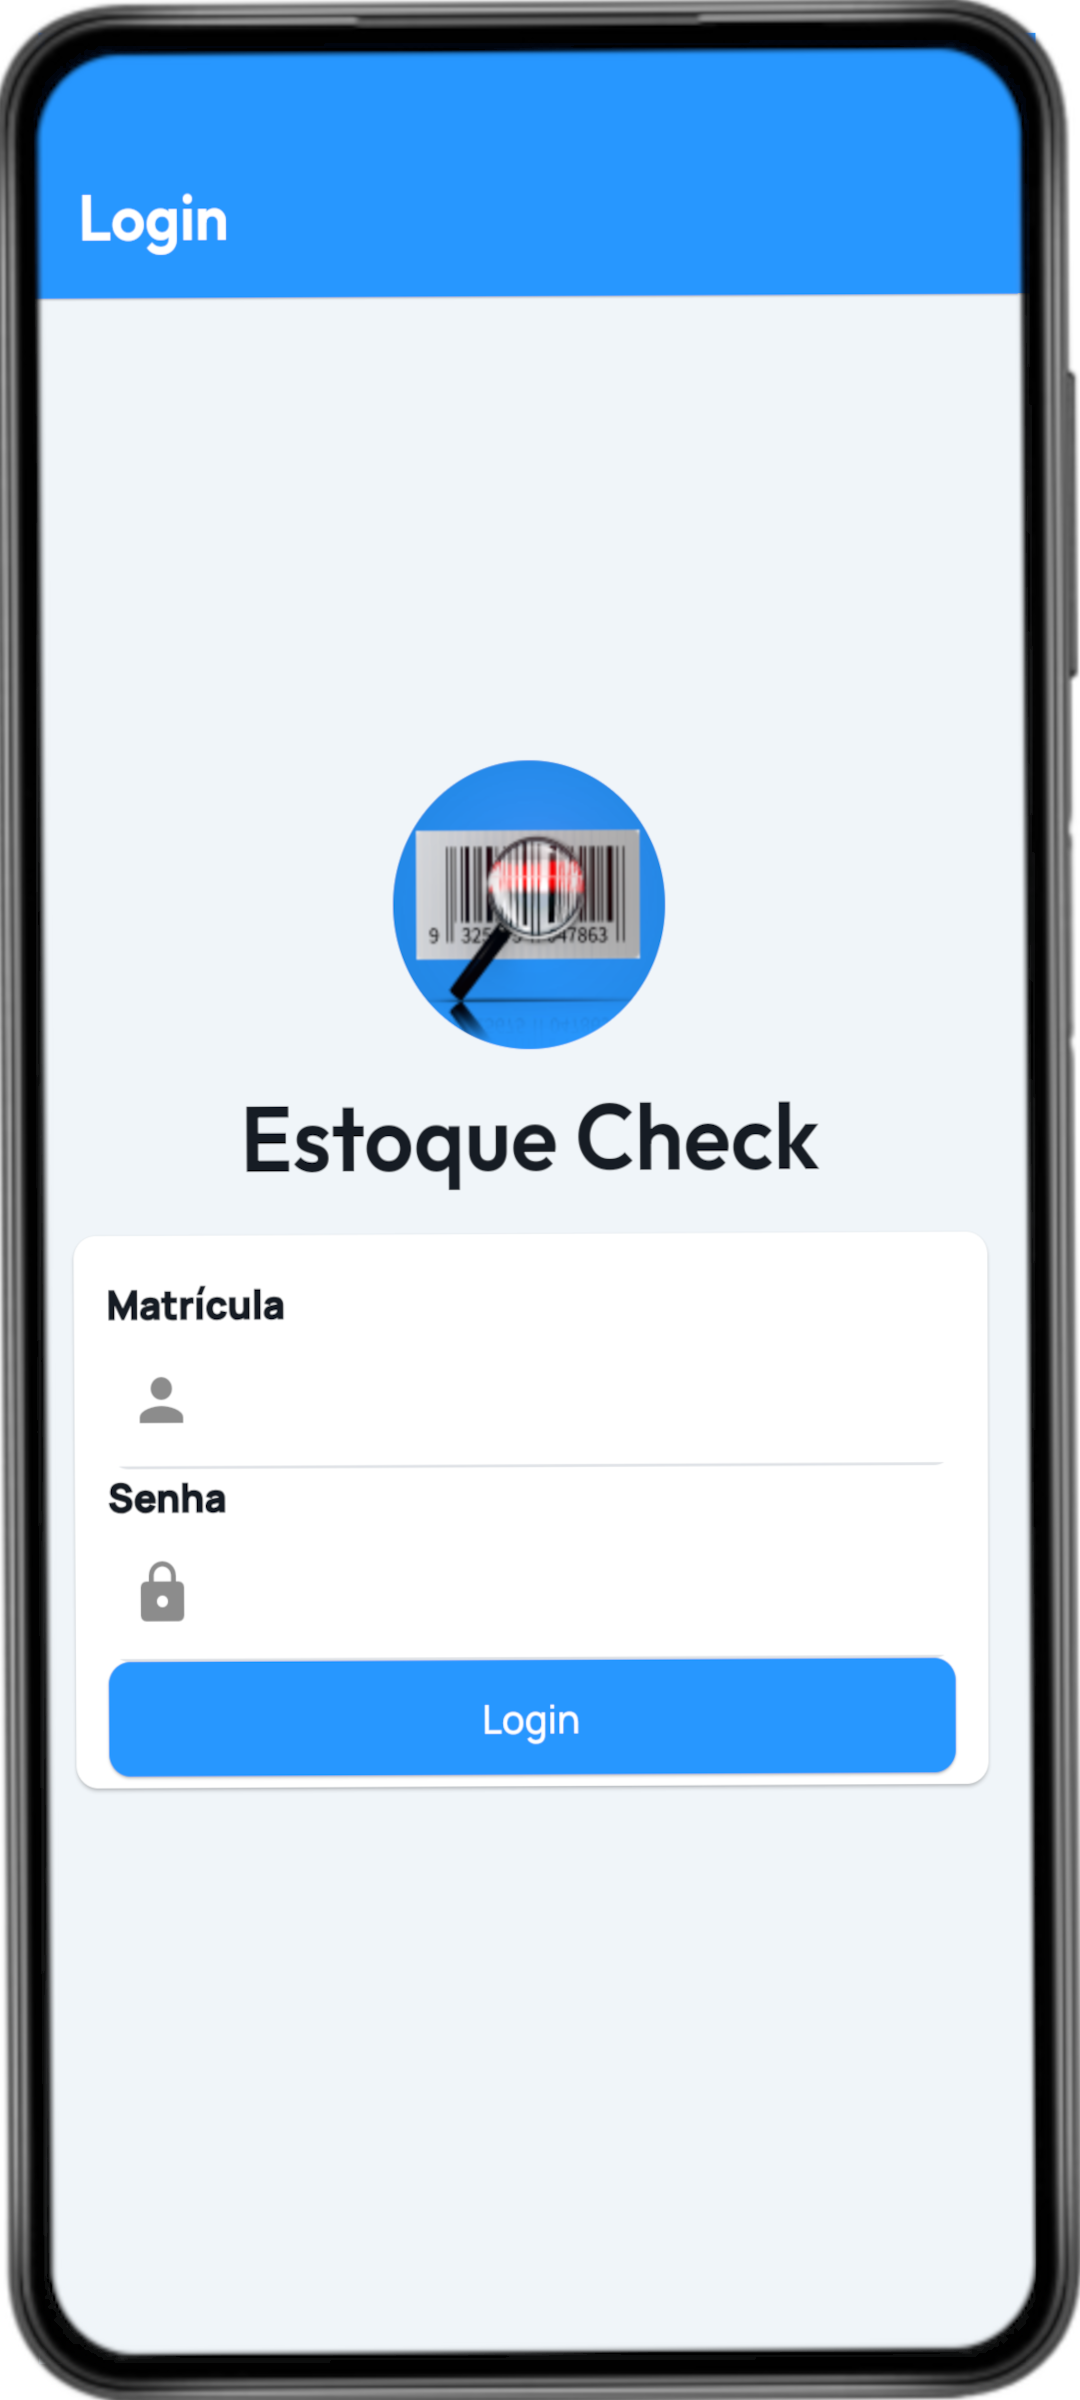
\includegraphics[width=0.15\textwidth]{imgs/login.png}
    }
    \quad
    \subfigure[Tela principal. \label{fig:homepage}]{
        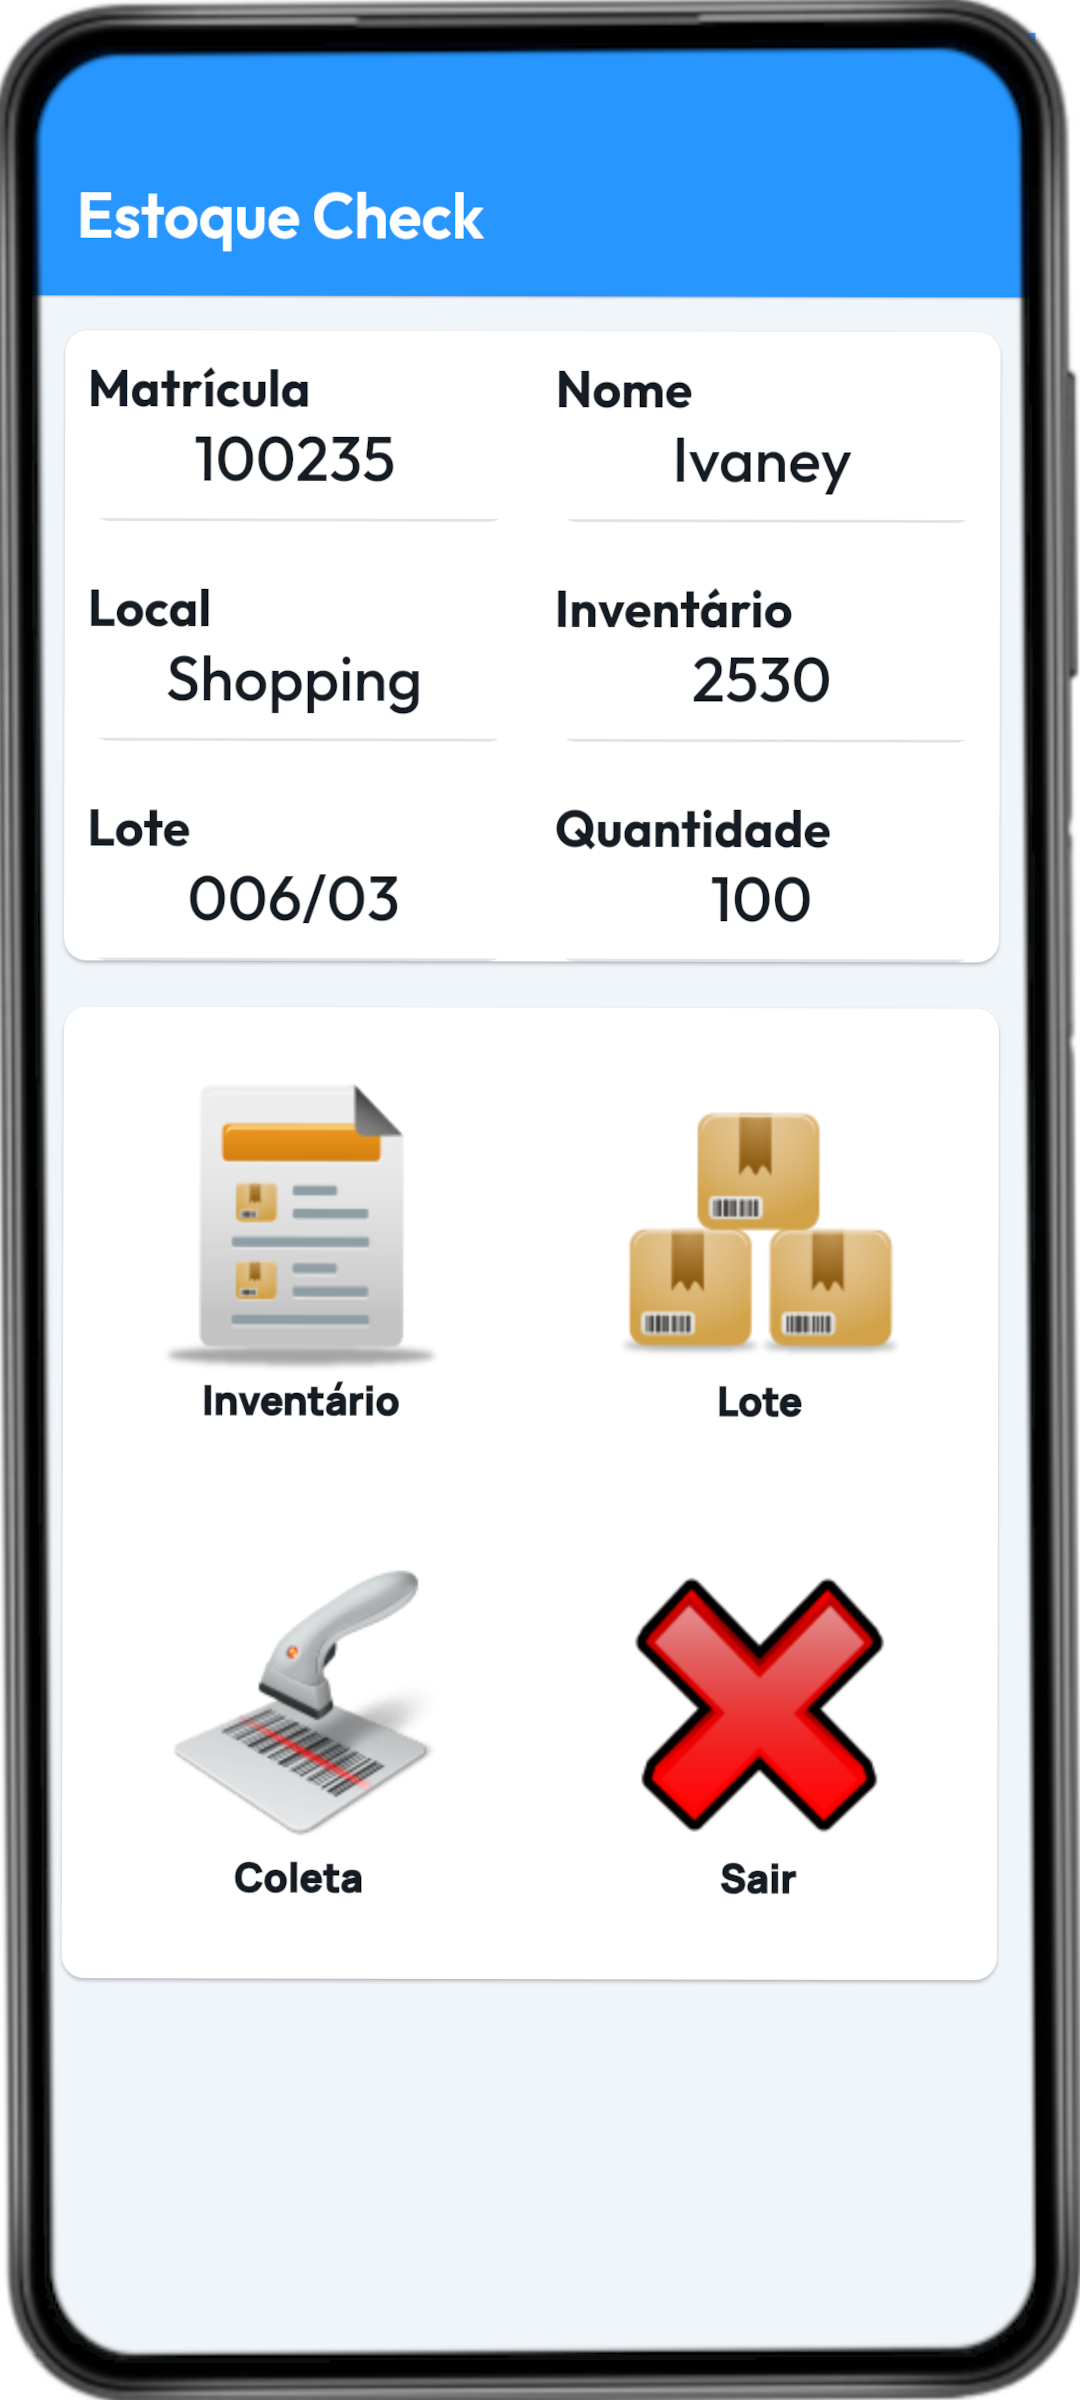
\includegraphics[width=0.15\textwidth]{imgs/homepage.png}
    }
    \quad
    \subfigure[Seleção de inventário.\label{fig:inventario}]{
        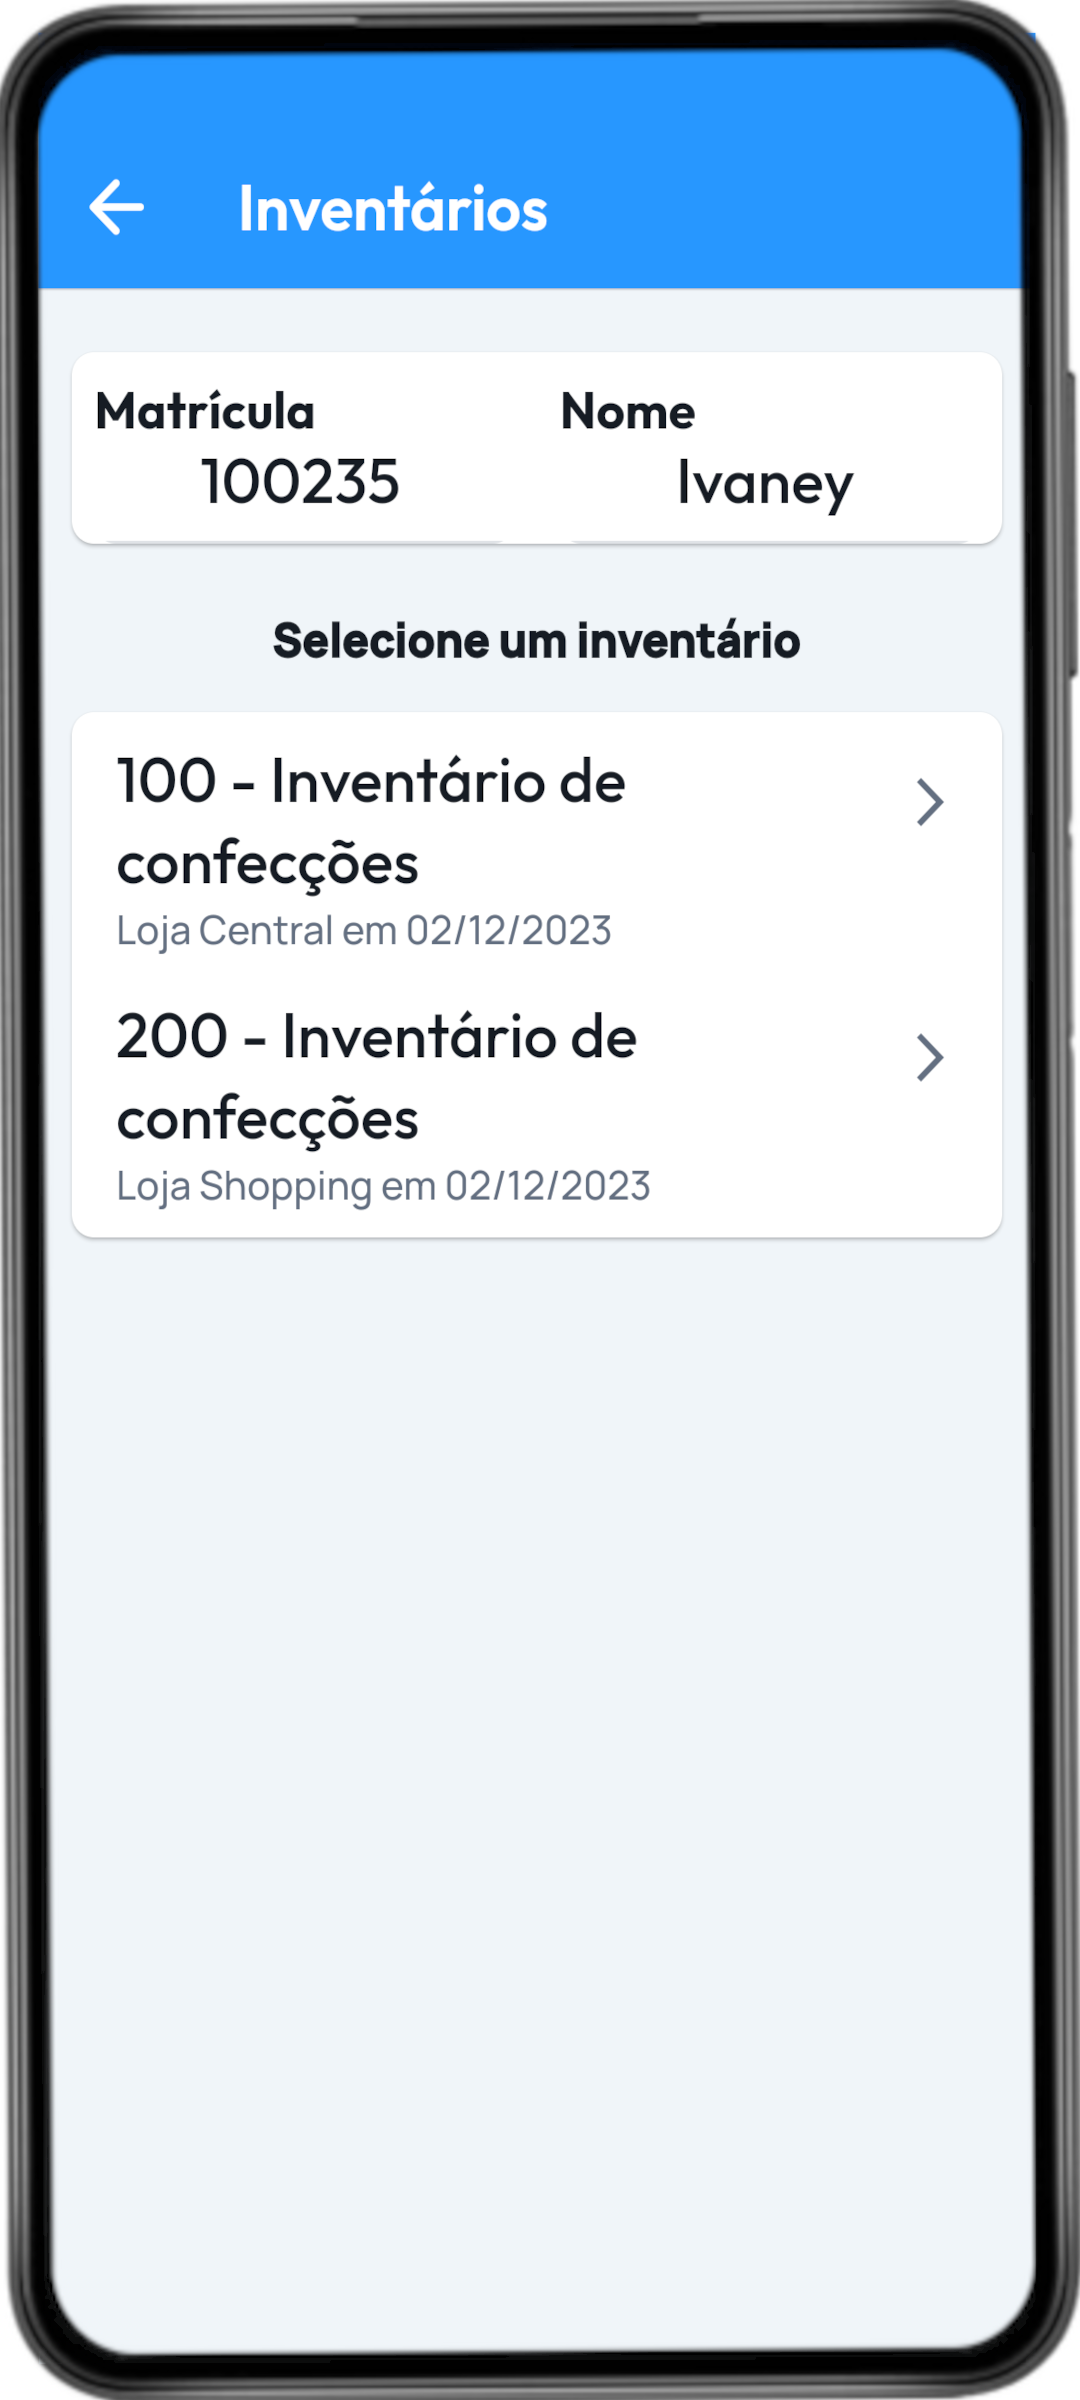
\includegraphics[width=0.15\textwidth]{imgs/inventario.png}
    }
    \quad
    \subfigure[Seleção de Lote.\label{fig:lote}]{
        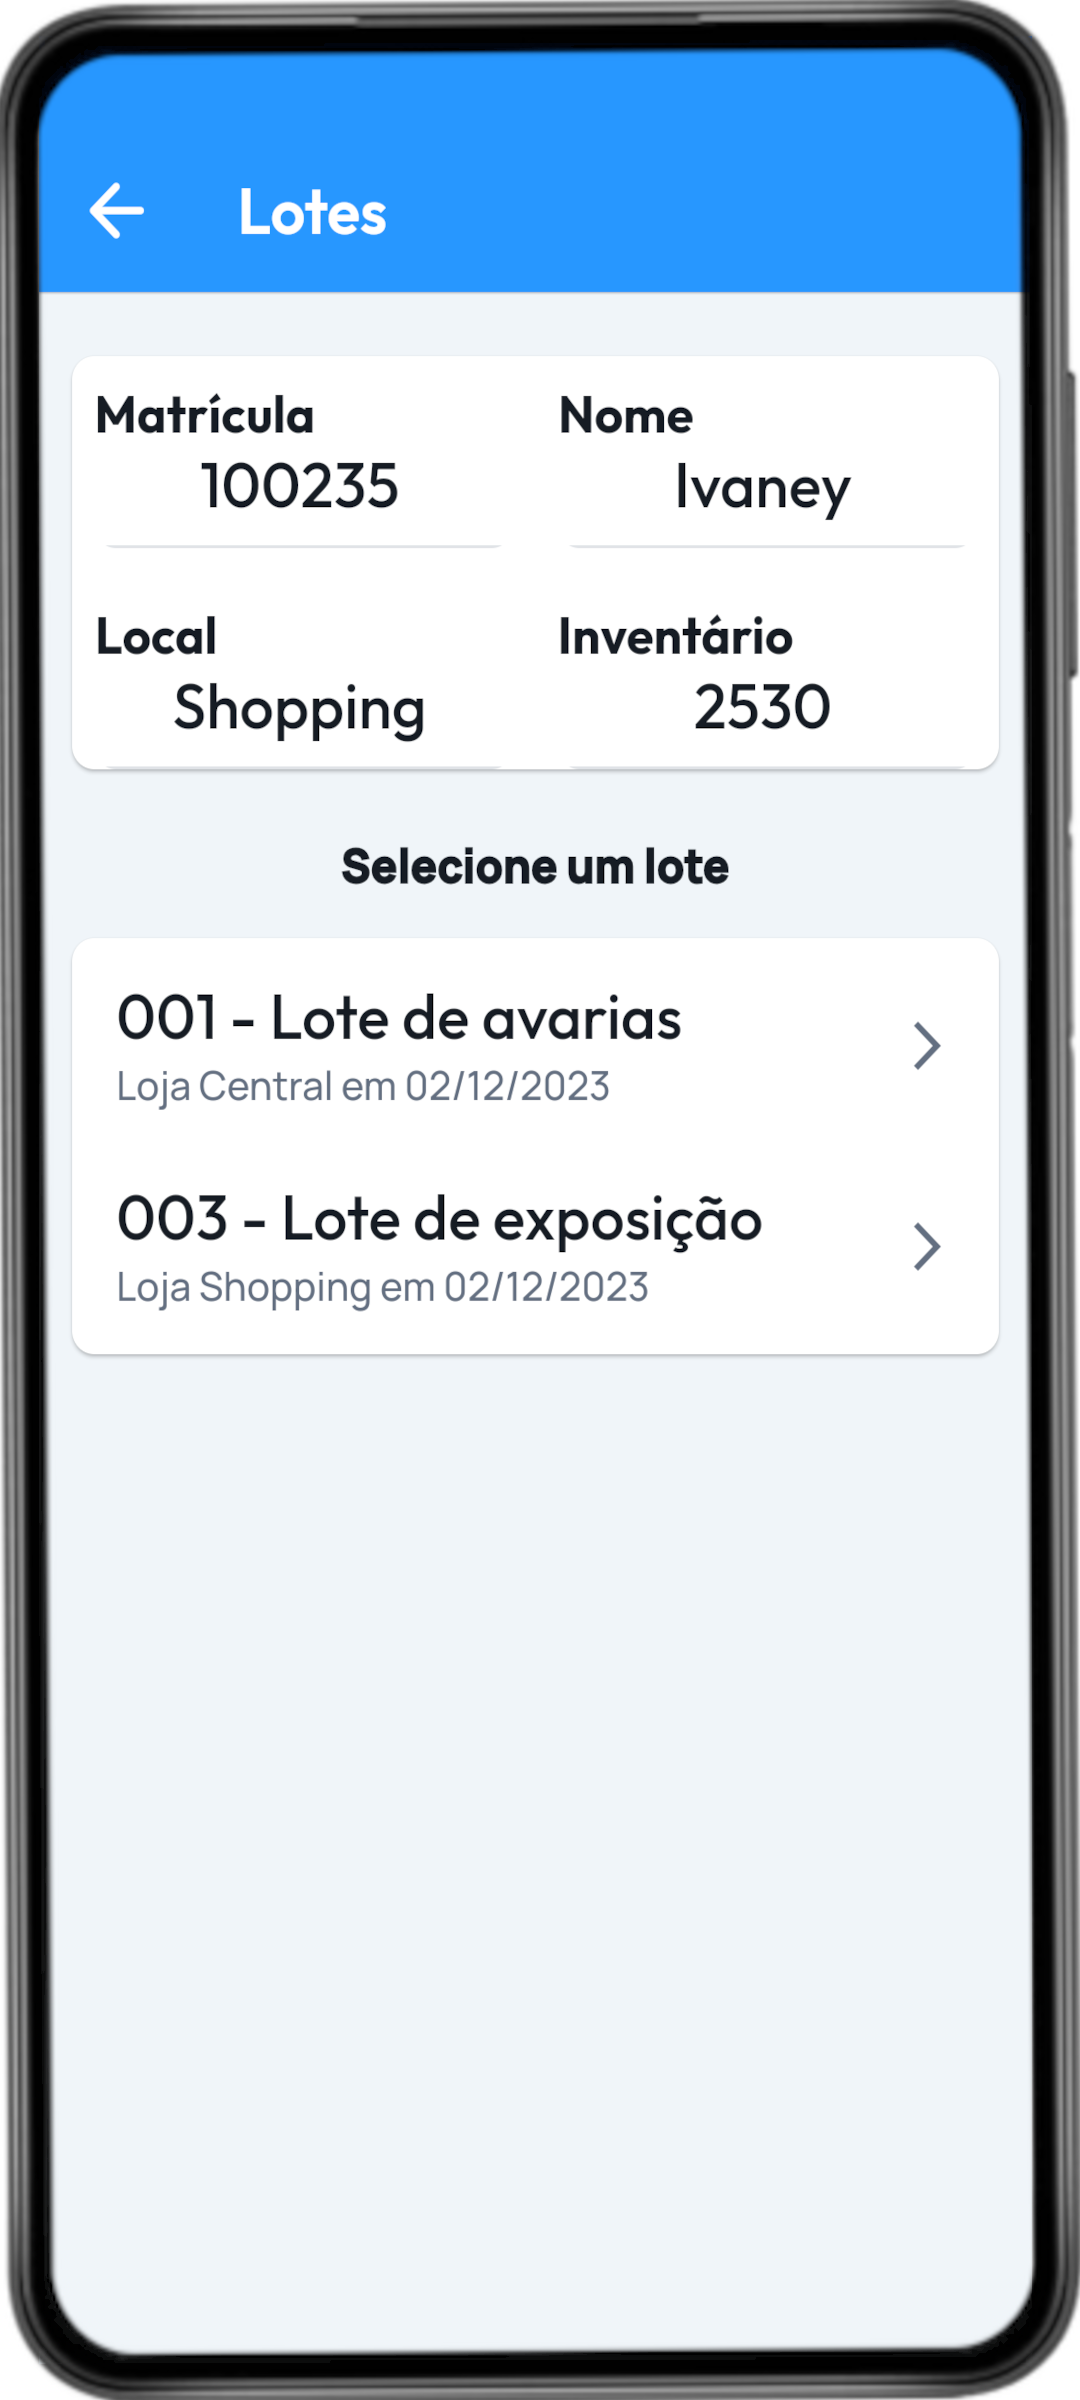
\includegraphics[width=0.15\textwidth]{imgs/lote.png}
    }
    \quad
    \subfigure[Coleta para contagem.\label{fig:coleta}]{
        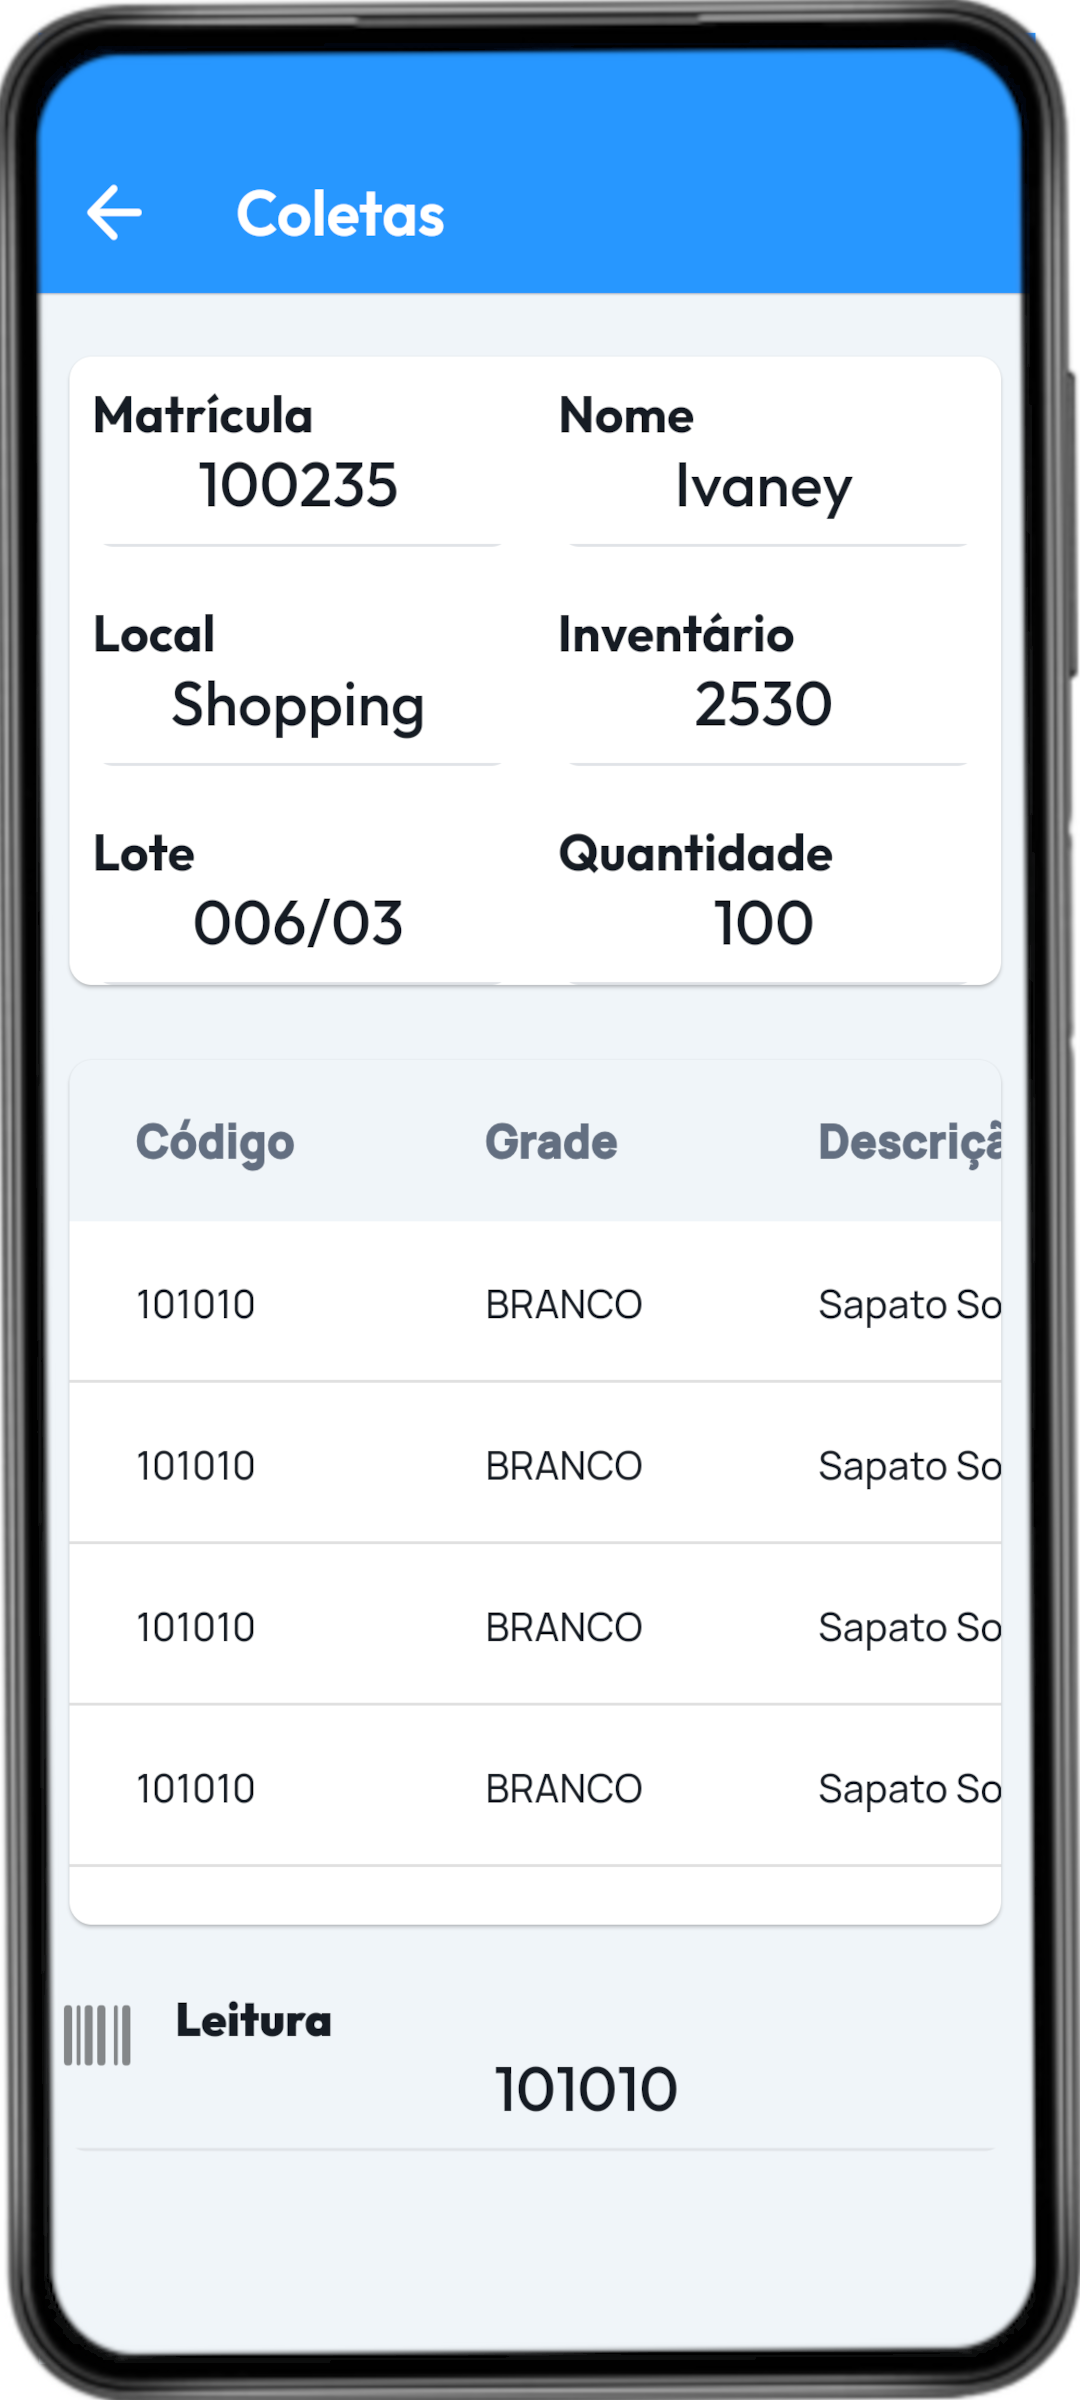
\includegraphics[width=0.15\textwidth]{imgs/coleta.png}
    }
    \label{fig:grupo01}
    \caption{Layout de telas para o aplicativo}
\label{fig:telas}
\end{figure}

A figura \ref{fig:telas} apresenta o layout das telas do aplicativo conforme descrito a seguir:

\begin{itemize}
    \item \textbf{Figura \ref{fig:login}}: temos a tela de login onde o usuário deve informar o usuário e senha para acessar o aplicativo. Lembrando que o usuário é autenticado usando as mesmas informações de acesso do ERP da empresa.
    \item \textbf{Figura \ref{fig:homepage}}: mostra a tela principal do aplicativo, onde o usuário pode selecionar o inventário que deseja realizar a contagem ou retomar uma contagem já iniciada. 
    \item \textbf{Figura \ref{fig:inventario}}: mostra a tela de seleção de inventário, onde o usuário pode visualizar os inventários disponíveis e selecionar o que deseja realizar a contagem. 
    \item \textbf{Figura \ref{fig:lote}}: exibe a tela de seleção de lote, onde o usuário pode ver os lotes disponíveis e escolher qual deseja contar. Um lote é um conjunto de produtos agrupados em um espaço físico específico, como, por exemplo, um palete, uma gôndola ou uma estante, e é identificado por um código e um código de barras. O auditor pode selecionar o lote lendo o código de barras.
    \item \textbf{Figura \ref{fig:coleta}}: mostra a tela de coleta para contagem, onde o usuário pode ver os produtos disponíveis no lote e registrar a quantidade contada de cada item. Ao finalizar a contagem, o usuário pode enviar os dados para o sistema de gestão da empresa. Nesse momento, a situação do lote é definida como fechado, podendo ser reaberto apenas pelo administrador.
\end{itemize}

Durante a contagem o administrador fica acompanhando o progresso das contagem e também pode configurar alerta para serem enviados aos auditores, informando sobre a proximidade do fim do inventário ou atrasos na contagem.

Após a conclusão da contagem, o administrador fecha o inventário. Os dados são validados por meio de uma análise estatística e, em seguida, processados para realizar ajustes gerenciais e fiscais do estoque.

\subsection{Aplicativos semelhantes}

\begin{table}[H]
    \centering
    \caption{Funcionalidades dos aplicativos semelhantes.}
    \label{tab:comparativos}
    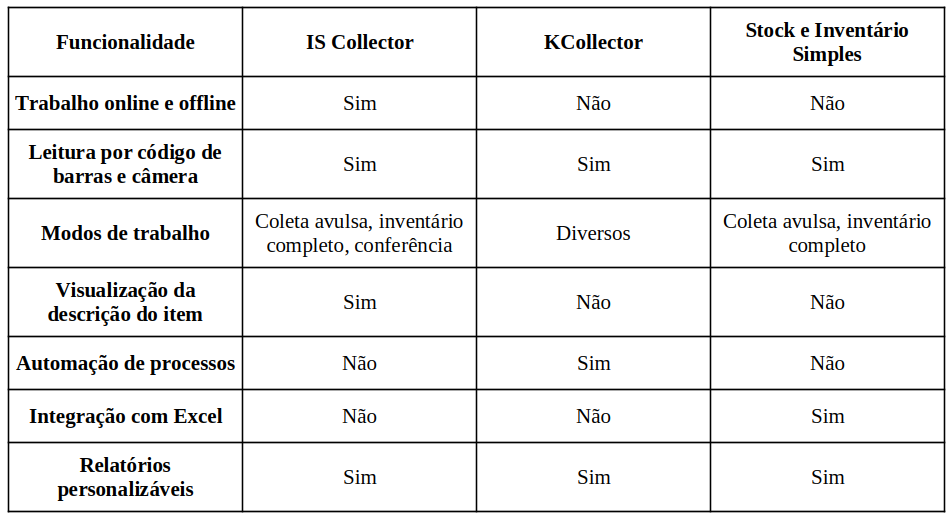
\includegraphics[width=1.0\textwidth]{tables/comparativo.png}
\end{table}

O IS Collector se destaca pela flexibilidade e abrangência de funções, ideal para empresas que exigem um alto nível de controle e automação no processo de inventário. O KCollector é a opção ideal para quem busca uma solução acessível e prática, que transforma o celular em um coletor eficiente. Já o Stock e Inventário Simples se destaca pela facilidade de uso e pelo gerenciamento completo do estoque, sendo uma ótima opção para iniciantes e pequenos negócios.

% Colocar aqui um parágrafo comparando o aplicativo do trabalho com os aplicativos pesquisados
O aplicativo do presente trabalho se destaca pela integração com o sistema de gestão da empresa, garantindo a consistência e a atualização em tempo real dos dados de estoque. Além disso, a interface intuitiva e as funcionalidades customizáveis proporcionam uma experiência de usuário eficiente e adaptável às necessidades específicas de cada empresa. A integração com tecnologias avançadas, como leitura de códigos de barras e alertas automatizados, eleva a eficácia do aplicativo, tornando-o uma solução completa e moderna para o controle de inventário.
